\documentclass[a4paper,14pt]{extarticle}
\usepackage[left=2.5cm, right=1.5cm, vmargin=2.5cm]{geometry}
\usepackage[utf8]{inputenc}
\usepackage[T2A]{fontenc}
\usepackage[russian]{babel}
\usepackage{graphicx}
\graphicspath{{pictures/}}
\usepackage{caption}
\usepackage{subcaption}
\usepackage{indentfirst}
\setlength\parindent{5ex}
\usepackage{fancyhdr}
\usepackage{booktabs}
\usepackage{siunitx} 
\usepackage{pgfplotstable}
\usepackage{amsmath}
\usepackage{autonum}
\usepackage{amsfonts}
\DeclareMathOperator{\sign}{sgn}
\newcommand{\gt}{\textgreater} % знак больше
\newcommand{\lt}{\textless}       % знак меньше
\DeclareGraphicsExtensions{.pdf,.png,.jpg}
\pagestyle{fancy}
\fancyhf{}
\rhead{\thepage}
\renewcommand{\headrulewidth}{0pt}

\fancypagestyle{plain}{ 
	\fancyhf{}
	\rhead{\thepage}}

\author{Никитин Илья}

\title{Отчет по лабораторной работе №2: "Дифракция Фраунгофера на решетке"}
\date{\today}

\begin{document}
	
	\maketitle
	\tableofcontents

	\section{Задачи}
		\begin{itemize}
			\item Собрать установку для наблюдения дифракции на отражающей дифракционной решетке, изучить дифракционную картину для различных решеток при различных углах падения света на решетку $\theta_i$, определить положения максимумов.
			\item Для каждой решеки определить число штрихов на единицу длины a.
			\item С помощью фотодиодного измерителя мощности измерить интенсивность света в максимумах для решетки, с помощью которой наблюдается наибольшее количество максимумов. Обработав полученную зависимость, определить угол скоса решетки $\gamma$
		\end{itemize}
	\section{Оборудование}
		\begin{itemize}
			\item Лазер с длиной волны испускаемого света 520 нм
			\item Отражающие дифракционные решетки с разными постоянными решетки
			\item Рулетка, закрепленная на стене
			\item Линейка
			\item Анализатор интенсивности падающего света
			\item Различная оптическая арматура
		\end{itemize}
	\section{Теория}
		\subsection{Дифракция на одной щели}
			Пусть края щели находятся в координатах $x = \pm b / 2$, где $b$ - ширина щели. На щель падает плоская монохроматическая волна с волновым вектором $k$ под углом $\theta_i$ к вектору нормали к решетке.
			
			\begin{figure}[h!]
				\centering
				\includegraphics[width=1\linewidth]{Diff1.png}
				\caption{Дифракция Фраунгофера на щели}
				\label{fig1}
			\end{figure}
			
			\newpage
			
			Разность фаз между волнами излучаемыми из координаты $x = 0$ и $x$ равна $\delta_1 = -k x (\sin{\theta} + sin{\theta_i})$. Получим:
			\begin{equation}
				E(\theta) \sim \int_{b/2}^{b/2}{\exp(-i \delta_1(x))dx} \sim \int_{b/2}^{b/2}{\exp(-i k x (\sin{\theta} + \sin{\theta_i})) dx}
			\end{equation}
			\begin{equation}
				E(\theta) \sim \frac{\sin(k b / 2 (\sin{\theta} + \sin{\theta_i})}{k b / 2 (\sin{\theta} + \sin{\theta_i}}
			\end{equation}
			\subsection{Дифракция на решетке с $N$ щелями}
			Разность хода между вторичными волнами, образованными соседними щелями равна $\delta = d k (\sin{\theta} + \sin{\theta_i})$, кроме того, поле, излучаемое щелью с номером $n$ равно $E_n = E_1 \exp(-i \delta n)$. Отсюда результирующее поле: 
			\begin{equation}
				E = E_1 * \sum_{0}^{N-1} \exp(-i \delta n) = E_1 \exp(i\delta(N/2 - 1)) \frac{\sin(N \delta /2)}{\sin(\delta /2)}
			\end{equation}
			Отсюда можно получить интенсивность:
			\begin{equation}
				I \sim E^2 \sim [\frac{\sin(k b / 2 (\sin{\theta} + \sin{\theta_i}))}{k b / 2 (\sin{\theta} + \sin{\theta_i})}]^2 [\frac{\sin(N k d / 2 (\sin{\theta} + sin{\theta_i}))}{\sin(k d / 2 (\sin{\theta} + sin{\theta_i}))}]^2
			\end{equation}
			Правый множитель отвечает за положение наблюдаемых максимумов, он же дает нам следующее условие:
			\begin{equation}
				d(\sin{\theta} + \sin{\theta_i}) = m \lambda,
			\end{equation}
			где $m$ - целое число, называемое порядком максимума. 
			\subsection{Дифракция на концентрирующей отражающей решетке}
			В концентрирующей отражающей решетке из-за геометрии изменится множитель $E_1(\theta)$, второй множитель останется тем же.
			\begin{equation}
				I \sim E^2 \sim [\frac{\sin(k b / 2 (\sin(\theta - \gamma) + \sin(\theta_i - \gamma)))}{k b / 2 (\sin(\theta - \gamma) + \sin(\theta_i - \gamma))}]^2 [\frac{\sin(N k d / 2 (\sin{\theta} + sin{\theta_i}))}{\sin(k d / 2 (\sin{\theta} + sin{\theta_i}))}]^2
			\end{equation}
			
			\begin{figure}[h!]
				\centering
				\includegraphics[width=1\linewidth]{Diff2.png}
				\caption{Схематичный рисунок установки}
				\label{fig2}
			\end{figure}
		
			Здесь нас будет интересовать первый, изменившийся множитель, который представляет из себя огибающую по интенсивности кривую.
			
			Угол, под которым налюдается максимум интенсивности, соответствует зеркальному отражению падающего света, называется углом блеска и определяется следующим выражением:
			\begin{equation}
				\phi_B = 2\gamma - \theta_i
			\end{equation}
			
	\section{Ход работы}
		\subsection{Определение числа штрихов дифракционных решеток}
			\subsubsection{Постановка эксперимента}
			На оптическом столе соберем следующую схему: закрепим дифракционные решетки напротив экрана, который представляет из себя стену с закрепленной рулеткой для измерения координат пучков на экране. Будем двигать лазер, изменяя углы падения луча на решетку и записывая полученные результаты. Повторим данный эксперимент для всех трех решеток.
			
			\begin{figure}[h!]
				\centering
				\includegraphics[width=1\linewidth]{Diff3.png}
				\caption{Схематичный рисунок установки}
				\label{fig0}
			\end{figure}
		
			\newpage
			
			\subsubsection{Результаты эксперимента}
				В результате эксперимента мы получили различные геометрические параметры нашей системы. Элементарно переходя от расстояний к углам, будем строить графики $\sin{\theta} + \sin{\theta_i}$ в зависимости от номера максимума $m$:
				
				\newpage
				
				\begin{figure}[h!]
					\centering
					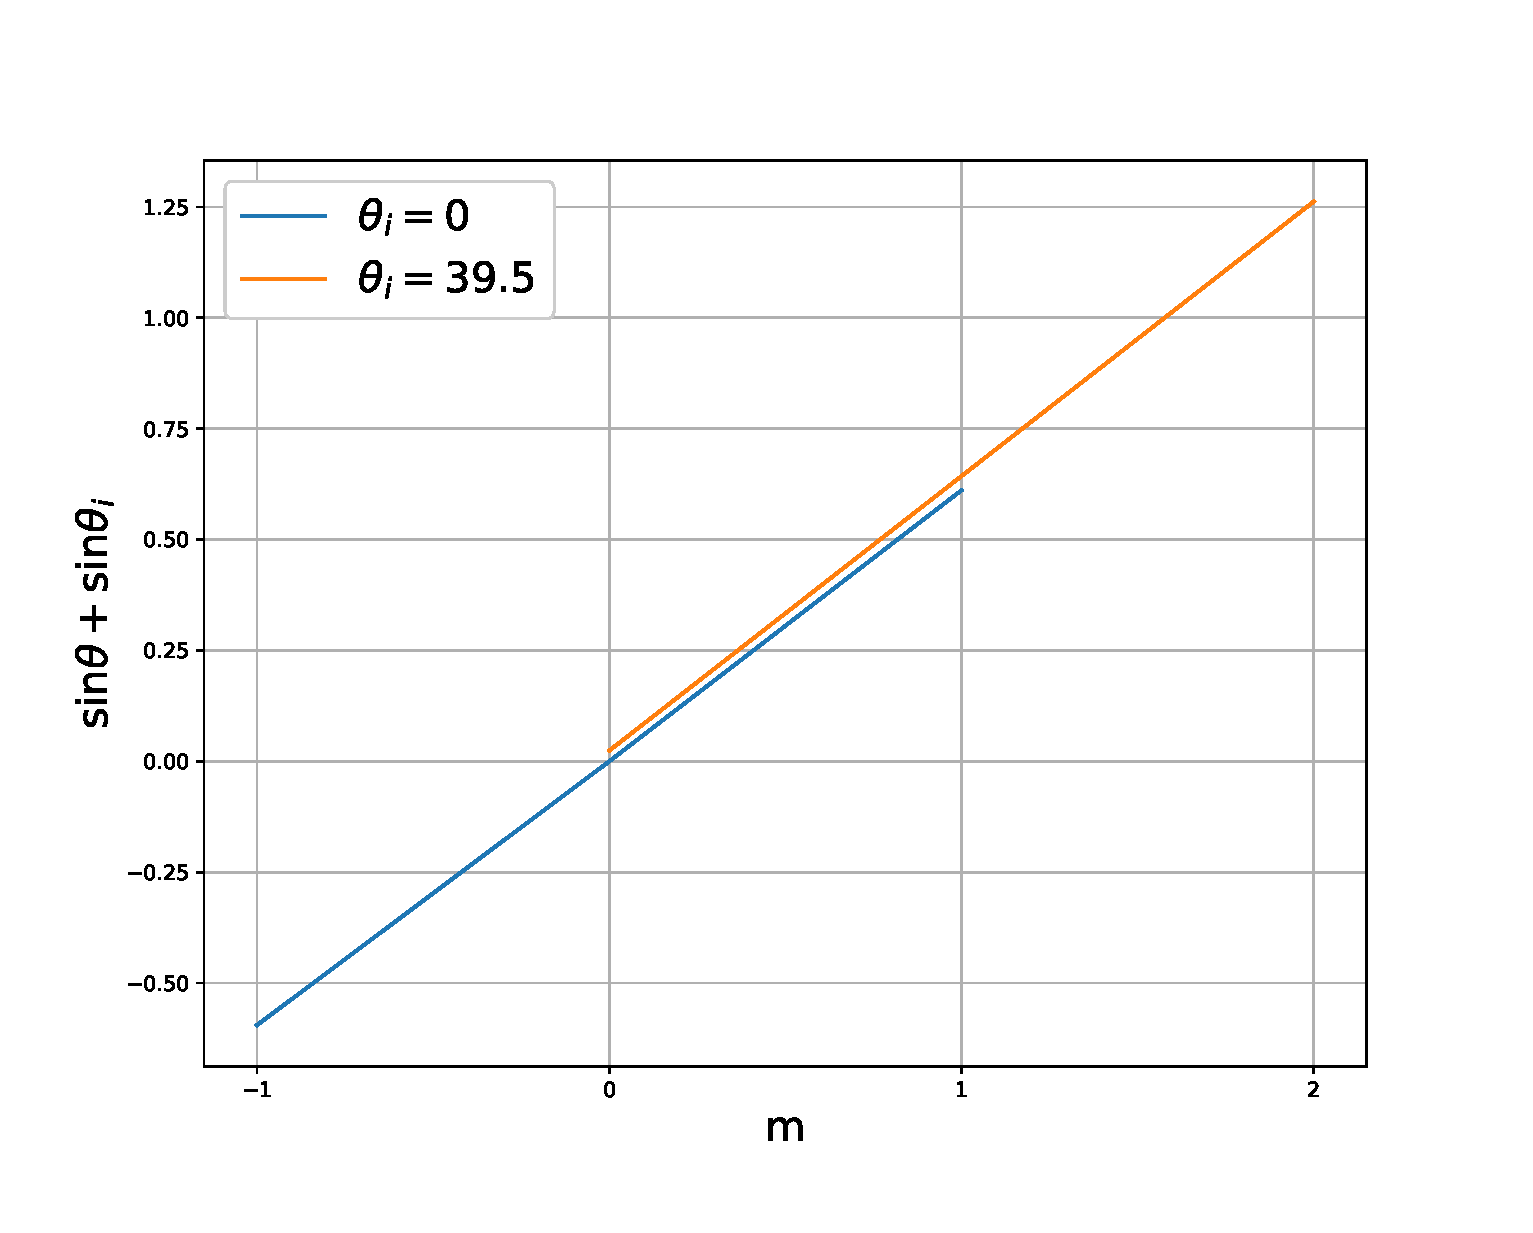
\includegraphics[width=1\linewidth]{Fraun1.eps}
					\caption{Зависимость суммы синусов от номера максимума для первой решетки}
					\label{fig3}
				\end{figure}
				
				\newpage
				
				\begin{figure}[h!]
					\centering
					\includegraphics[width=1\linewidth]{Fraun2.eps}
					\caption{Зависимость суммы синусов от номера максимума для второй решетки}
					\label{fig4}
				\end{figure}
				
				\newpage
				
				\begin{figure}[h!]
					\centering
					\includegraphics[width=1\linewidth]{Fraun3.eps}
					\caption{Зависимость суммы синусов от номера максимума для третьей решетки}
					\label{fig5}
				\end{figure}				
				
				Для каждой решетки выразим количество штрихов через усредненный коэффициент наклона получившихся прямых $N_{slits} = \alpha / \lambda * 10^{-3}$ штрихов на мм. Получим:
				\begin{equation}
					\begin{cases}
						N_{slits 1} \approx 1180 \pm 25 \text{мм}^{-1}, \\
						N_{slits 2} \approx 520 \pm 25 \text{мм}^{-1}, \\
						N_{slits 3} \approx 265 \pm 25 \text{мм}^{-1}. \\
					\end{cases}
				\end{equation}
				
				\newpage
				
		\subsection{Определение угла скоса решетки}
			\subsubsection{Постановка эксперимента}
			Для решетки с наибольшим количеством максимумов в предыдущую постановку эксперимента добавим анализатор интенсивности, измеряющий интенсивность видимых максимумов. Построив график, попробуем профитировать его огибающей, упомянутой в теоретической части.
			\subsubsection{Результаты эксперимента}
			Получаем вот такой график (интенсивность нормирована на интенсивность максимума), который был подогнан по единственному параметру $\gamma$ -- углу скоса отражающей дифракционной решетки.
			
			\newpage
			
			\begin{figure}[h!]
				\centering
				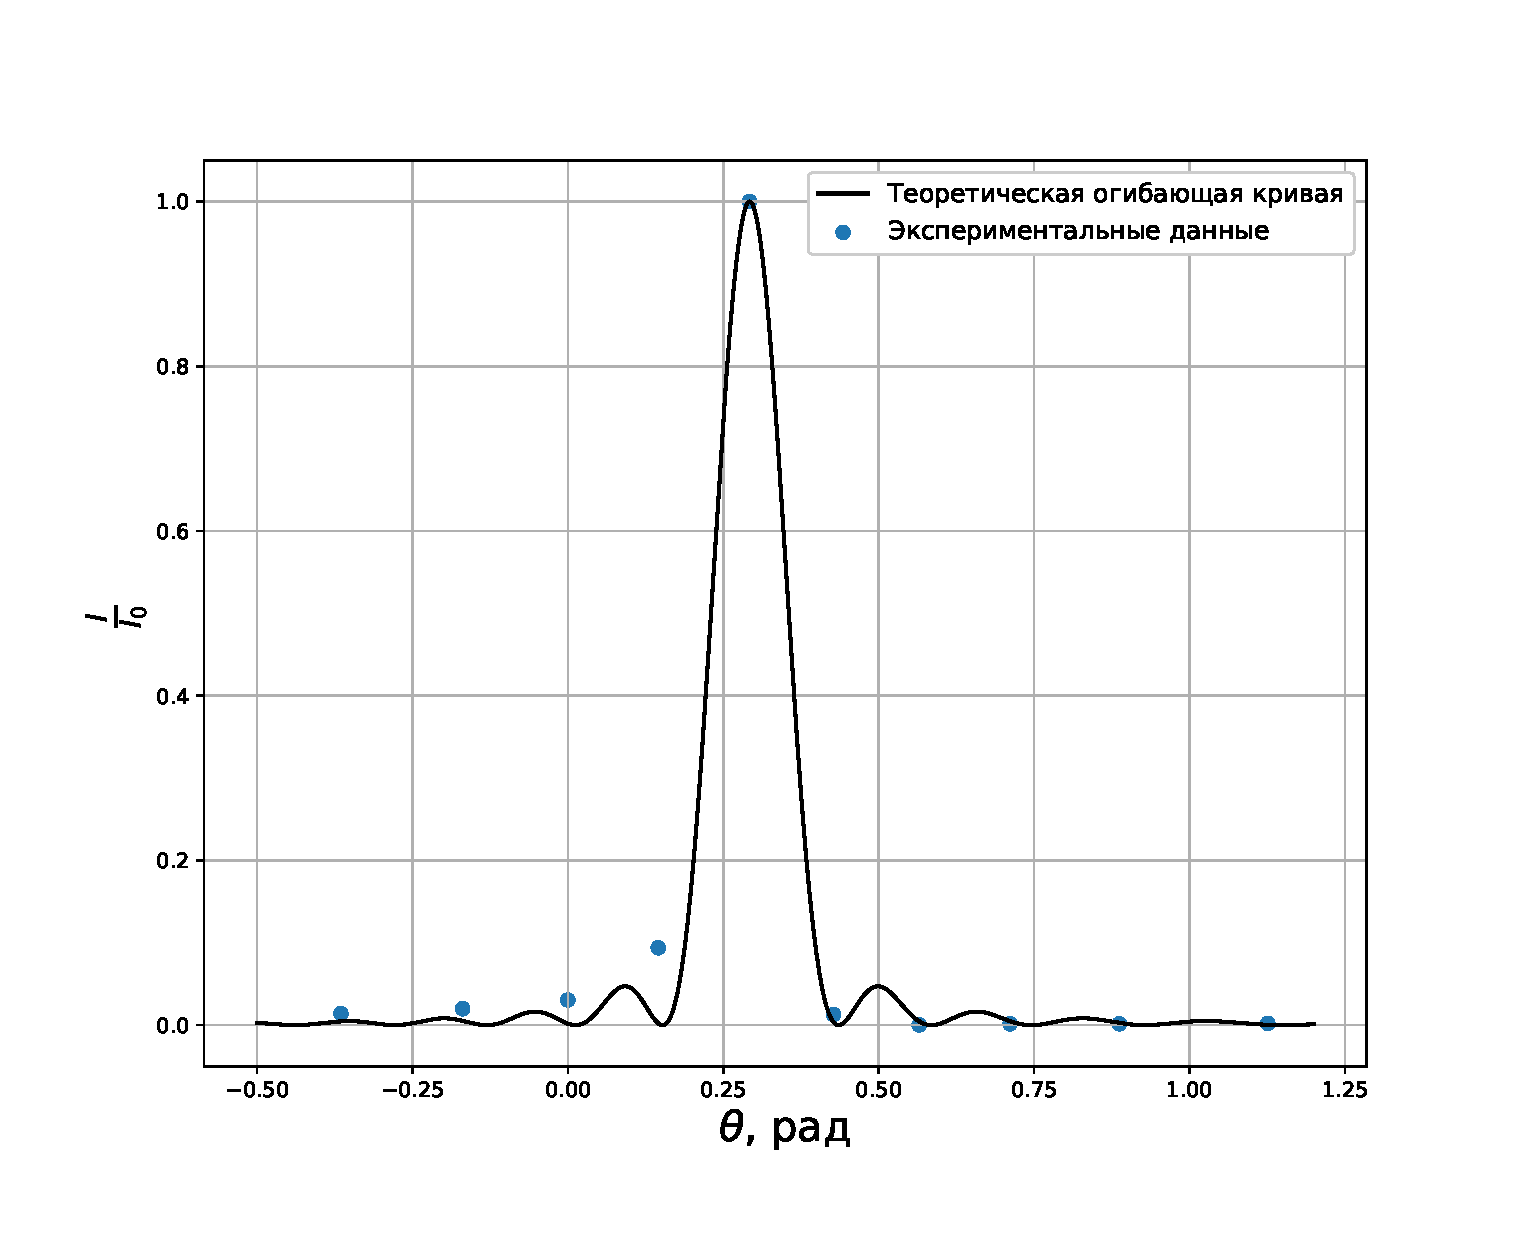
\includegraphics[width=1\linewidth]{Fraun4.eps}
				\caption{Зависимость интенсивности от угла $\theta$ для третьей решетки}
				\label{fig6}
			\end{figure}
			
			В результате фитирования было получено значение $\gamma = 0.14 \pm 0.02$ рад
	\section{Выводы}
		\begin{itemize}
			\item С помощью предложенной установки были получены значения числа штрихов на единицу длины для каждой решетки. 
			\begin{equation}
				\begin{cases}
					N_{slits 1} \approx 1180 \pm 25 \text{ мм}^{-1}, \\
					N_{slits 2} \approx 520 \pm 25 \text{ мм}^{-1}, \\
					N_{slits 3} \approx 265 \pm 25 \text{ мм}^{-1}. \\
				\end{cases}
			\end{equation}
			\item Нами было исследовано распределение интенсивности отраженного от концетрирующей решетки света и для конкретной решетки получено значение угла скоса $\gamma = 0.14 \pm 0.02$ рад
		\end{itemize}
\end{document}